\documentclass[tikz,border=10pt]{standalone}
\begin{document}
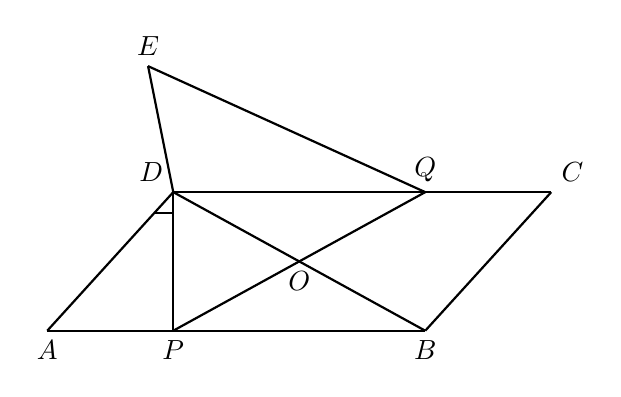
\begin{tikzpicture}[scale=0.8,thick]
\coordinate (A) at (0,0);
\coordinate (P) at (2,0);
\coordinate (B) at (6,0);
\coordinate (C) at (8,2.2);
\coordinate (D) at (2,2.2);
\coordinate (Q) at (6,2.2);
\coordinate (E) at (1.6,4.2);
\coordinate (O) at (4,1.1);

\draw (A) -- (B);
\draw (B) -- (C);
\draw (C) -- (Q);
\draw (Q) -- (D);
\draw (D) -- (A);
\draw (D) -- (P);
\draw (D) -- (B);
\draw (P) -- (Q);
\draw (E) -- (D);
\draw (E) -- (Q);

% right angle mark at D between DA and DP
\draw ([shift={(-0.3,-0.33)}]D) -- ([shift={(-0.3,-0.33)}]D) -- ++(0.3,0) -- ++(0,-0.33);

\foreach \p/\pos in {A/below,P/below,B/below,C/above right,D/above left,Q/above,E/above,O/below}
  \node[\pos] at (\p) {$\p$};
\end{tikzpicture}
\end{document}
